%! Author = adrienkoumgangtegantchouang
%! Date = 08/06/25


\chapter{System Design}\label{ch:system-design}


This chapter presents the architectural and structural design of the Smart News Aggregator \& Reader Personalization Platform.
It includes a high-level system architecture, database modeling strategy, UML class diagrams, and mockups of key user interfaces.


\section{Architecture Overview}\label{sec:architecture-overview}

The platform is built using a \textbf{modular and layered architecture} to separate concerns and ensure maintainability, performance, and scalability.
It integrates multiple technologies:

\subsection{Key Components}\label{subsec:key-components}

\begin{itemize}
    \item \textbf{Frontend (React + TypeScript)}: Handles UI, user interaction, API communication and Token-based authentication.
    \item \textbf{Backend (Flask + Flask-RESTX)}: RESTful API with Blueprint organization, JWT authentication with RS256 and Logging and error handling.
    \item \textbf{Document Database (MongoDB)}: Stores user profiles, articles, comments, and logs.
    Supports complex queries and aggregation pipelines.
    \item \textbf{Key-Value Store (Redis)}: Caches trending articles and recent queries.
    Session tracking.
    \item \textbf{External APIs}: Article data sources such as CurrentsAPI, NewsData, NYTimes, Guardian.
\end{itemize}


\section{System Architecture Diagram}\label{sec:system-architecture-diagram}

The architecture is divided into four layers:
\begin{itemize}
    \item \textbf{Client Layer}: Browser-based React frontend
    \item \textbf{Application Layer}: Flask server handling HTTP requests, routing, and validation
    \item \textbf{Data Layer}: MongoDB for structured content, Redis for quick key access
    \item \textbf{External Sources}: Third-party APIs for news ingestion
\end{itemize}


\begin{figure}[!h]
    \centering
    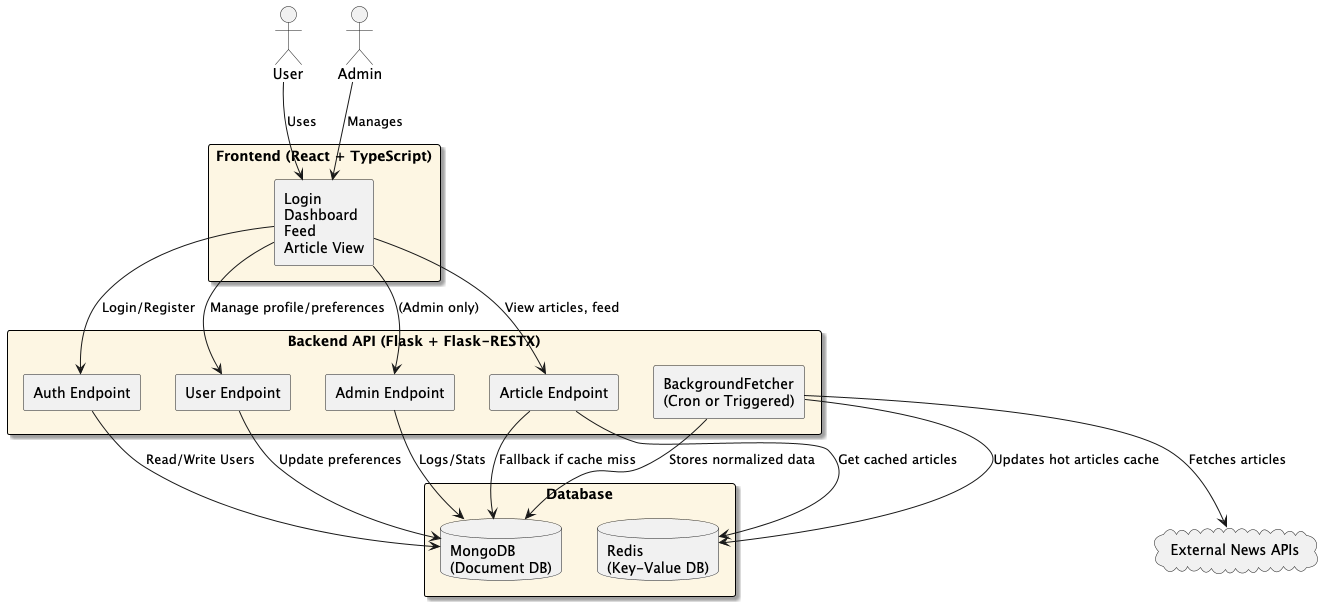
\includegraphics[width=1.1\textwidth]{chapters/chapter_03/system-architecture-smart-news-aggregator}
    \caption{Use Case Diagram: Systen}
    \label{fig:use-case-diagram-system}
\end{figure}

\subsection{Client Layer (Frontend)}\label{subsec:client-layer-frontend}

At the forefront is the \textbf{Client Layer}, which consists of a web-based frontend developed using React and TypeScript.
This layer handles the user interface, manages routing, and communicates with the backend API through Axios.
JWT tokens are stored in the browser’s localStorage for session management.
Users interact with interfaces such as login, registration, the personalized news feed, article detail views, and, for administrators, a dedicated dashboard.

\subsection{Application Layer (Flask Backend)}\label{subsec:application-layer-flask-backend}

The \textbf{Application Layer} is built on Flask with Flask-RESTX to expose RESTful endpoints in a modular architecture.
This layer is responsible for authenticating users using asymmetric JWT (RS256), routing client requests to appropriate service handlers, and managing background tasks like scheduled fetching of articles.
It includes modules like auth\_endpoint, user\_endpoint, article\_endpoint, and admin\_endpoint, as well as libraries for handling authentication keys and logging system events into MongoDB\@.

\subsection{Data Layer}\label{subsec:data-layer}

The \textbf{Data Layer} integrates two complementary NoSQL technologies.
MongoDB, as a document-oriented database, is used to store structured collections such as users, articles, comments, preferences, and system logs.
It supports advanced aggregation pipelines and enables efficient historical analysis.
Redis, on the other hand, serves as a key-value store optimized for performance.
It caches the latest articles, manages trending topics, and supports rate limiting.
Redis ensures low-latency data access and reduces the load on MongoDB for repetitive queries.

\subsection{External APIs Layer}\label{subsec:external-apis-layer}

At the periphery, the \textbf{External APIs Layer} includes third-party news services like MediaStack, CurrentsAPI, NewsData, the New York Times API, and the Guardian API\@.
A background fetcher service, either scheduled or triggered, connects to these APIs, retrieves articles, normalizes the data, and saves the cleaned results into MongoDB\@.
This ensures that the content database is continuously updated with fresh news.

\vspace{2cm}

The data flow follows a secure and performance-driven path.
When a user logs in, they are authenticated via JWT, and the token is returned in the Authorization header.
The frontend then retrieves the latest articles by calling the /article/latest endpoint.
If the content is cached in Redis, it is served directly; otherwise, Flask queries MongoDB. Meanwhile, the background fetcher periodically updates the article repository.
Personalized recommendations are generated by combining user preferences with MongoDB aggregations and Redis-cached data.
Administrators can monitor platform activity and user engagement via metrics obtained through aggregation queries stored in MongoDB\@.

\section{UML Class Diagram}\label{sec:uml-class-diagram}

\begin{figure}[!h]
    \centering
    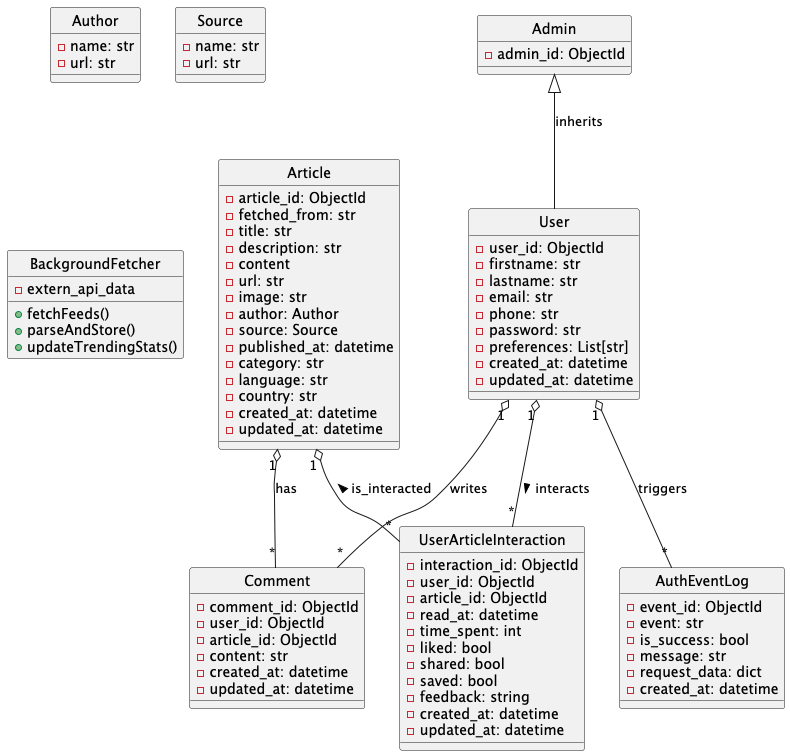
\includegraphics[width=1\textwidth]{chapters/chapter_03/uml-class-diagram}
    \caption{Use Case Diagram: Systen}
    \label{fig:uml-class-diagram}
\end{figure}


\section{Database Modeling}\label{sec:database-modeling}

\subsection{Document-Oriented Schema (MongoDB)}\label{subsec:document-oriented-schema-mongodb}


MongoDB stores structured documents for core domain entities.
Each entity is represented as a collection with JSON-like documents.
The key collections are:

\begin{itemize}
    \item Users Collection
\end{itemize}

\begin{lstlisting}[language=json]
{
  "_id": ObjectId,
  "email": "user@example.com",
  "password": "hashed_password",
  "first_name": "Alice",
  "last_name": "Smith",
  "created_at": ISODate,
  "preferences": {
    "categories": ["technology", "sports"],
    "languages": ["en"],
    "sources": ["NYTimes", "Guardian"]
  }
}
\end{lstlisting}


\begin{itemize}
    \item Articles Collection
\end{itemize}

\begin{lstlisting}[language=json]
{
  "_id": ObjectId,
  "extern_id": "nyt-123456",
  "title": "Breaking News",
  "content": "Full article content...",
  "author": "Journalist Name",
  "source": "NYTimes",
  "url": "https://...",
  "image_url": "https://...",
  "published_at": ISODate,
  "category": "technology",
  "language": "en",
  "country": "us"
}
\end{lstlisting}

\begin{itemize}
    \item User Articles Interactions Collection
\end{itemize}

\begin{lstlisting}[language=json]
{
  "_id": ObjectId,
  "user_id": ObjectId,
  "article_id": ObjectId,
  "read_at": ISODate,
  "time_spent": 120,
  "liked": true,
  "shared": false,
  "saved": false,
  "feedback": "Interesting article on AI trends."
}
\end{lstlisting}

\begin{itemize}
    \item Comments Collection
\end{itemize}

\begin{lstlisting}[language=json]
{
  "_id": ObjectId,
  "user_id": ObjectId,
  "article_id": ObjectId,
  "content": "This article was really informative.",
  "created_at": ISODate,
  "replies": [
    {
      "user_id": ObjectId,
      "content": "I agree!",
      "created_at": ISODate
    }
  ]
}
\end{lstlisting}

\begin{itemize}
    \item Logs Collection
\end{itemize}

\begin{lstlisting}[language=json]
{
  "_id": ObjectId,
  "event": "login",
  "user_id": ObjectId,
  "is_success": true,
  "request_data": {
    "method": "POST",
    "url": "/api/auth/login",
    "headers": { ... },
    "body": { ... }
  },
  "message": "Login successful!",
  "created_at": ISODate
}
\end{lstlisting}


\subsection{Key-Value Cache (Redis)}\label{subsec:key-value-cache-redis}



\section{UI Wireframes and Mockups}\label{sec:ui-wireframes-and-mockups}

\subsection{Authentication Screens}\label{subsec:authentication-screens}

\begin{figure}[!h]
    \centering
    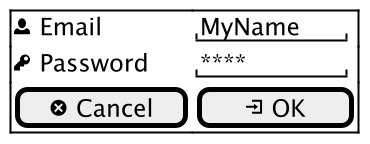
\includegraphics[width=0.7\textwidth]{chapters/chapter_03/login-wireframes}
    \caption{Use Case Diagram: Systen}
    \label{fig:login-wireframes}
\end{figure}

\begin{figure}[!h]
    \centering
    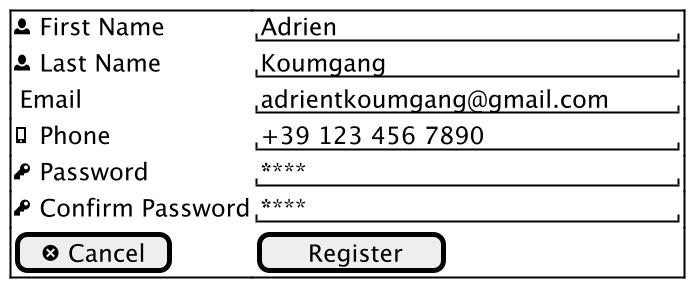
\includegraphics[width=0.7\textwidth]{chapters/chapter_03/registration-wireframes}
    \caption{Use Case Diagram: Systen}
    \label{fig:login-wireframes}
\end{figure}


\subsection{Article Feed View}\label{subsec:article-feed-view}


